\documentclass{article}
\usepackage{graphicx}
\usepackage{placeins}


\begin{document}
\begin{titlepage}
   \vspace*{\stretch{1.0}}
   \begin{center}
      \Large\textbf{Supplemental Figures}\\
      \vspace{1em}
      \Large{Chemotherapy weakly contributes to predicted neoantigen expression in ovarian cancer} \\
      \vspace{1em}
     \large\textit{Timothy O'Donnell, Elizabeth L. Christie, Arun Ahuja, Jacqueline Buros, B. Arman Aksoy, David D. L. Bowtell, Alexandra Snyder, Jeff Hammerbacher}
    % \large\textit{O’Donnell et al.}
   \end{center}
   \vspace*{\stretch{2.0}}
\end{titlepage}

% See http://tex.stackexchange.com/questions/168169/options-for-supplementary-materials-in-preprint-version-revtex-arxiv
\setcounter{equation}{0}
\setcounter{figure}{0}
\setcounter{table}{0}
\makeatletter
\renewcommand{\theequation}{S\arabic{equation}}
\renewcommand{\thefigure}{S\arabic{figure}}

\begin{figure}
\centering
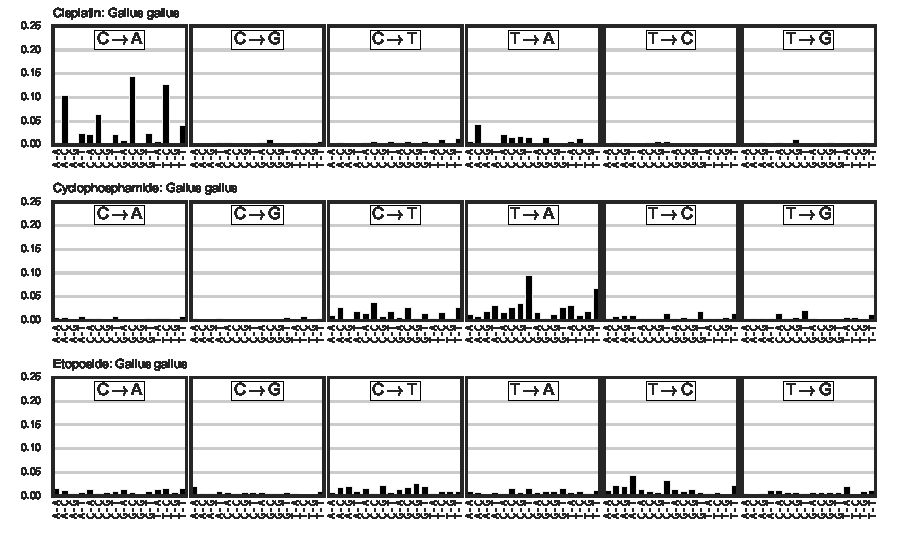
\includegraphics[scale=1.0]{../figures/extracted_signatures_chicken.pdf}
\caption{Mutational signatures extracted from Szikriszt et al.~\cite{Szikriszt_2016}}
\label{fig:supp_extracted_signatures_chicken}
\end{figure}

\begin{figure}
\centering
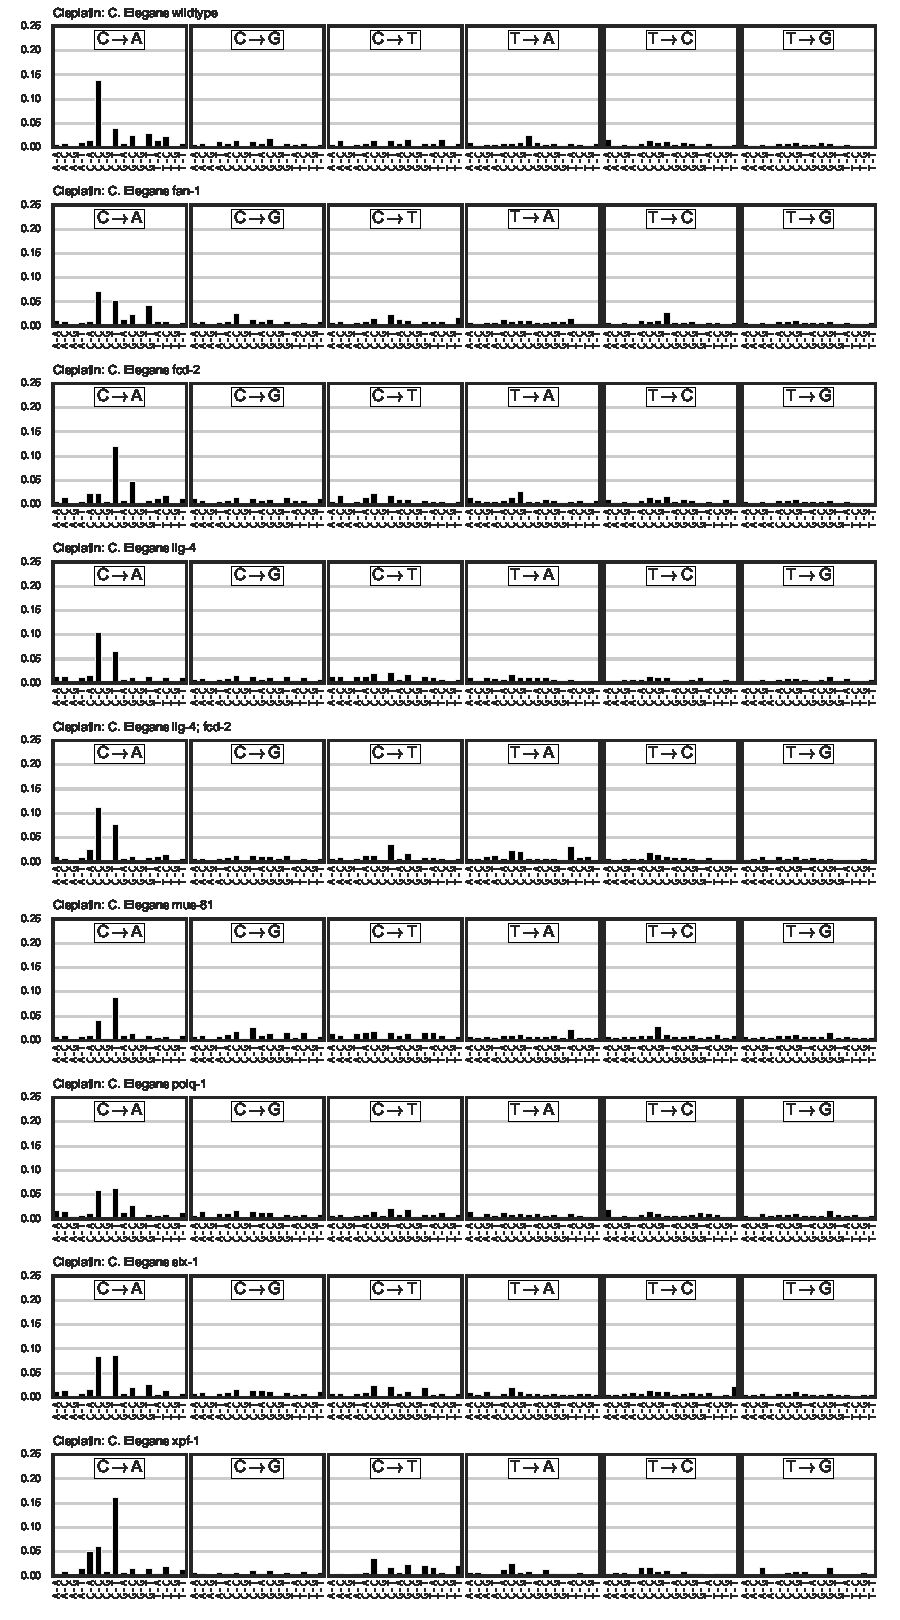
\includegraphics[scale=1.0]{../figures/extracted_signatures_worm.pdf}
\caption{Mutational signature extracted from Meier et al.~\cite{Meier_2014}}
\label{fig:supp_extracted_signatures_worm}
\end{figure}

\begin{figure}
\centering
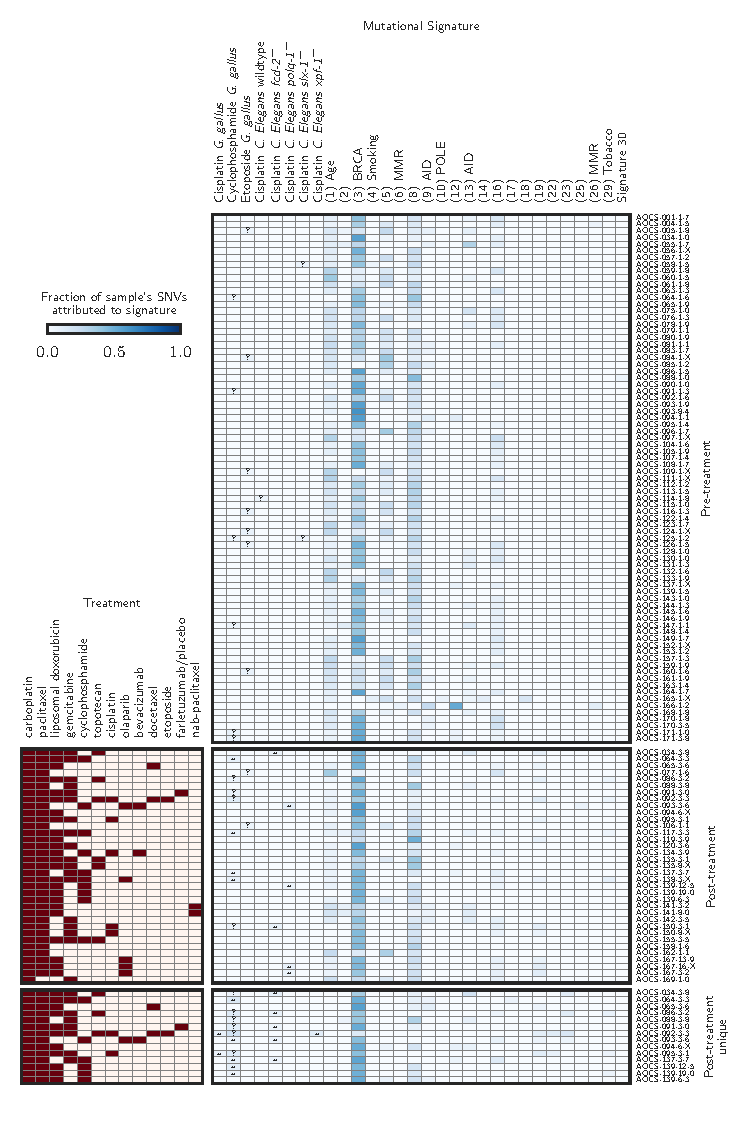
\includegraphics[scale=1.0]{../figures/supplementary_signatures.pdf}
\caption{\textbf{Detected mutational signatures across all samples.} The symbols are as in main text Figure~1. The top and middle panels show the signature deconvolutions for all pre- and post-treatment samples, respectively. The bottom panel shows deconvolutions for the mutations unique to the paired post-treatment samples, requiring high coverage and no variant reads in the donor-matched pre-treatment sample.}
\label{fig:supp_signatures}
\end{figure}

\begin{figure}
\centering
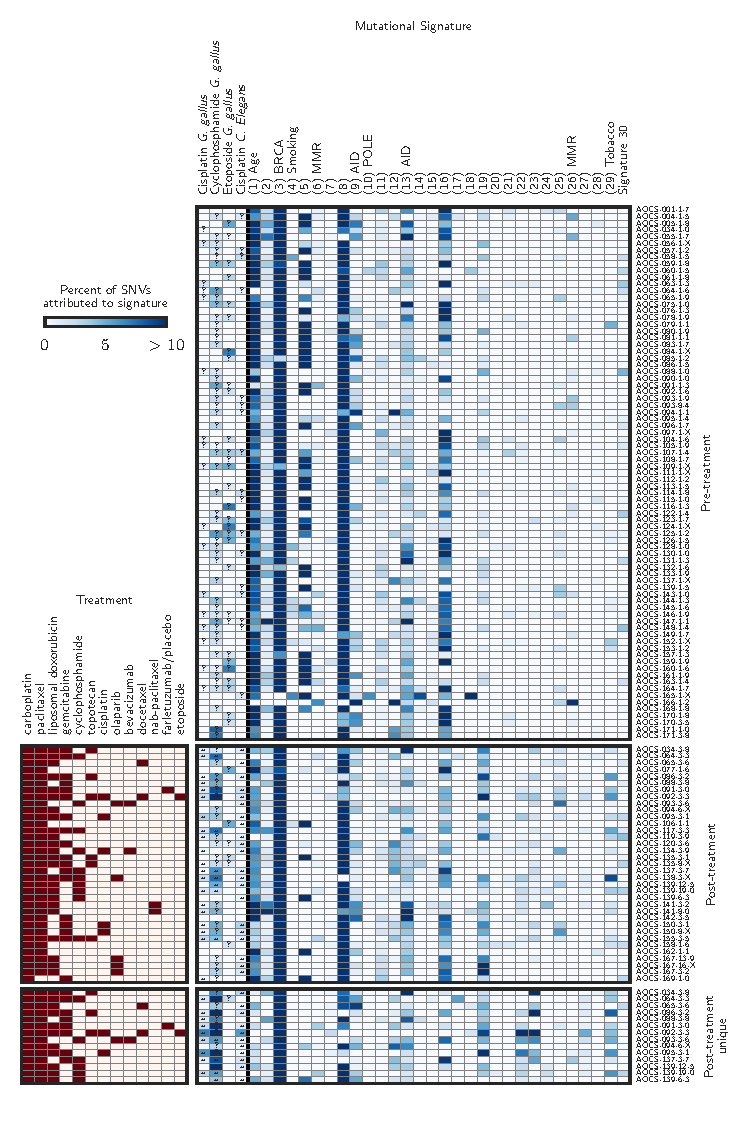
\includegraphics[scale=1.0]{../figures/supplementary_signatures_no_cutoff.pdf}
\caption{\textbf{Mutational signature deconvolutions without any threshold of detection.} Here, signatures accounting for less than the 6\% recommended detection threshold are included.}
\label{fig:supplementary_signatures_no_cutoff}
\end{figure}

\begin{figure}
\centering
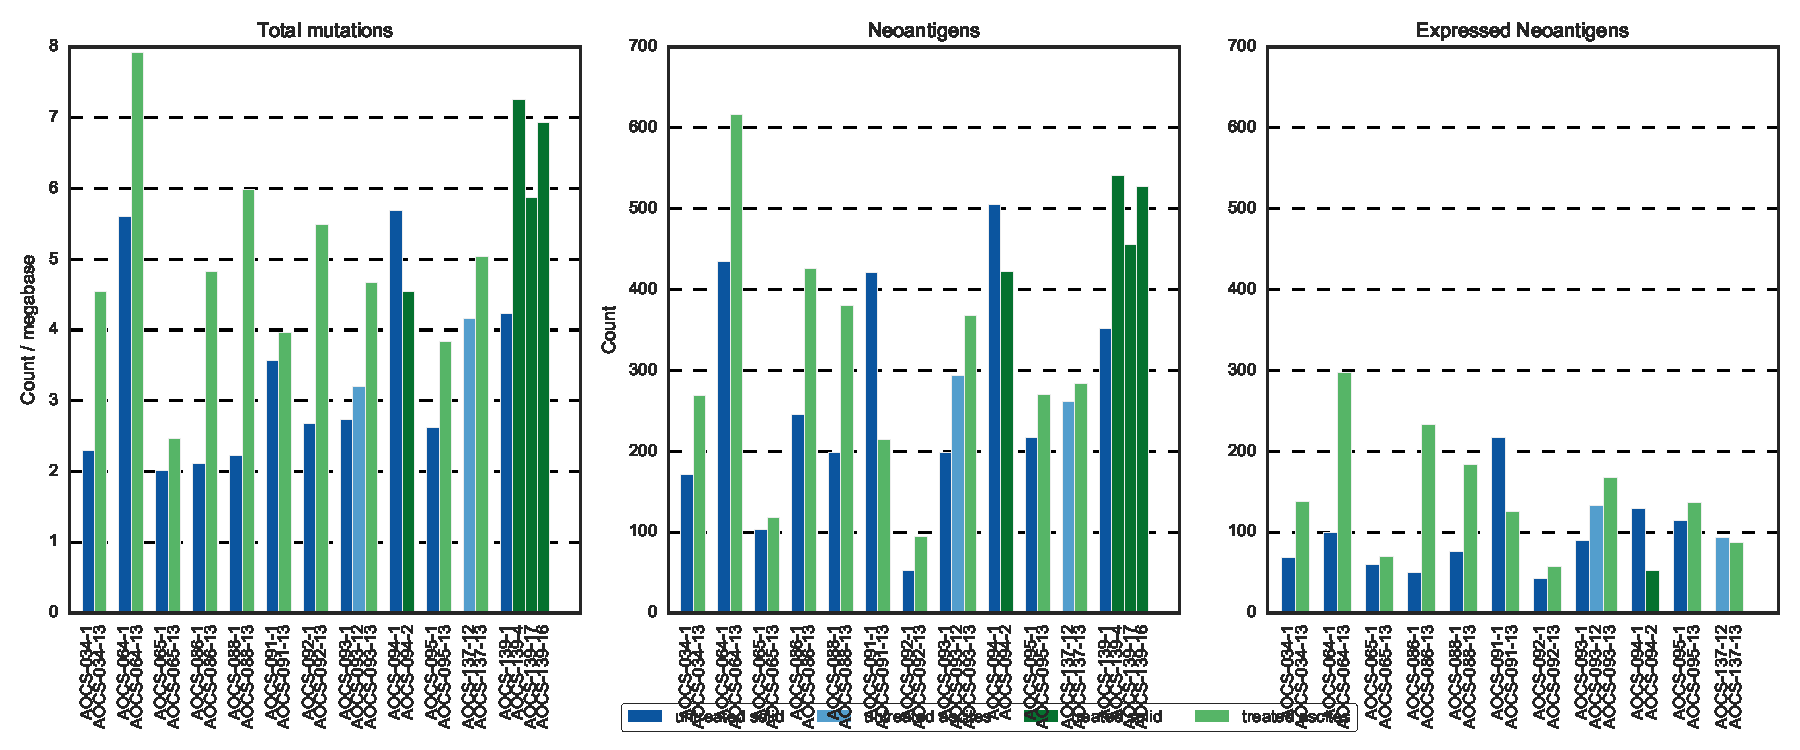
\includegraphics[scale=1.0]{../figures/paired_counts.pdf}
\caption{Mutations, neoantigens, and expressed neoantigens for donor-matched primary/untreated and relapse/treated samples.}
\label{fig:supp_paired}
\end{figure}

\begin{figure}[htbp]
\centering
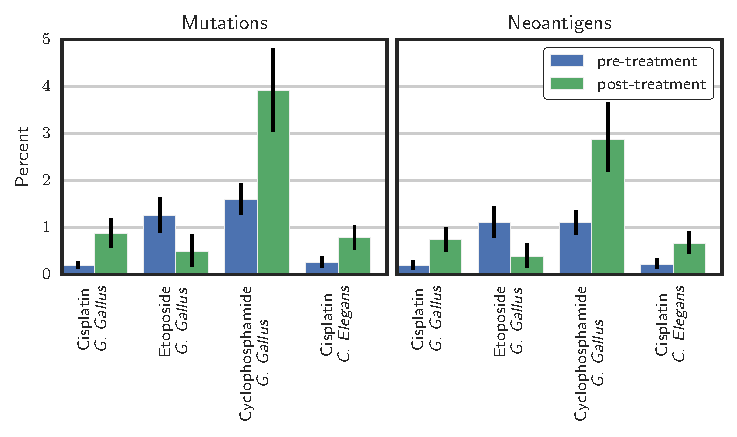
\includegraphics[scale=1.0]{../figures/sources_of_mutations_and_neoantigens_ungrouped.pdf}
\caption{\textbf{Contribution of chemotherapy SNV signatures.} The fraction of each sample's mutations, neoantigens, and expressed neoantigens attributed to putative chemotherapy signatures is shown. Bars give the mean, and points indicate individual samples.}
\label{fig:sourcesungrouped}
\end{figure}

\newpage
\FloatBarrier

\bibliography{bmc_article} 
\bibliographystyle{ieeetr}

\end{document}